\section{Results}

\begin{figure}[ht]
\center
  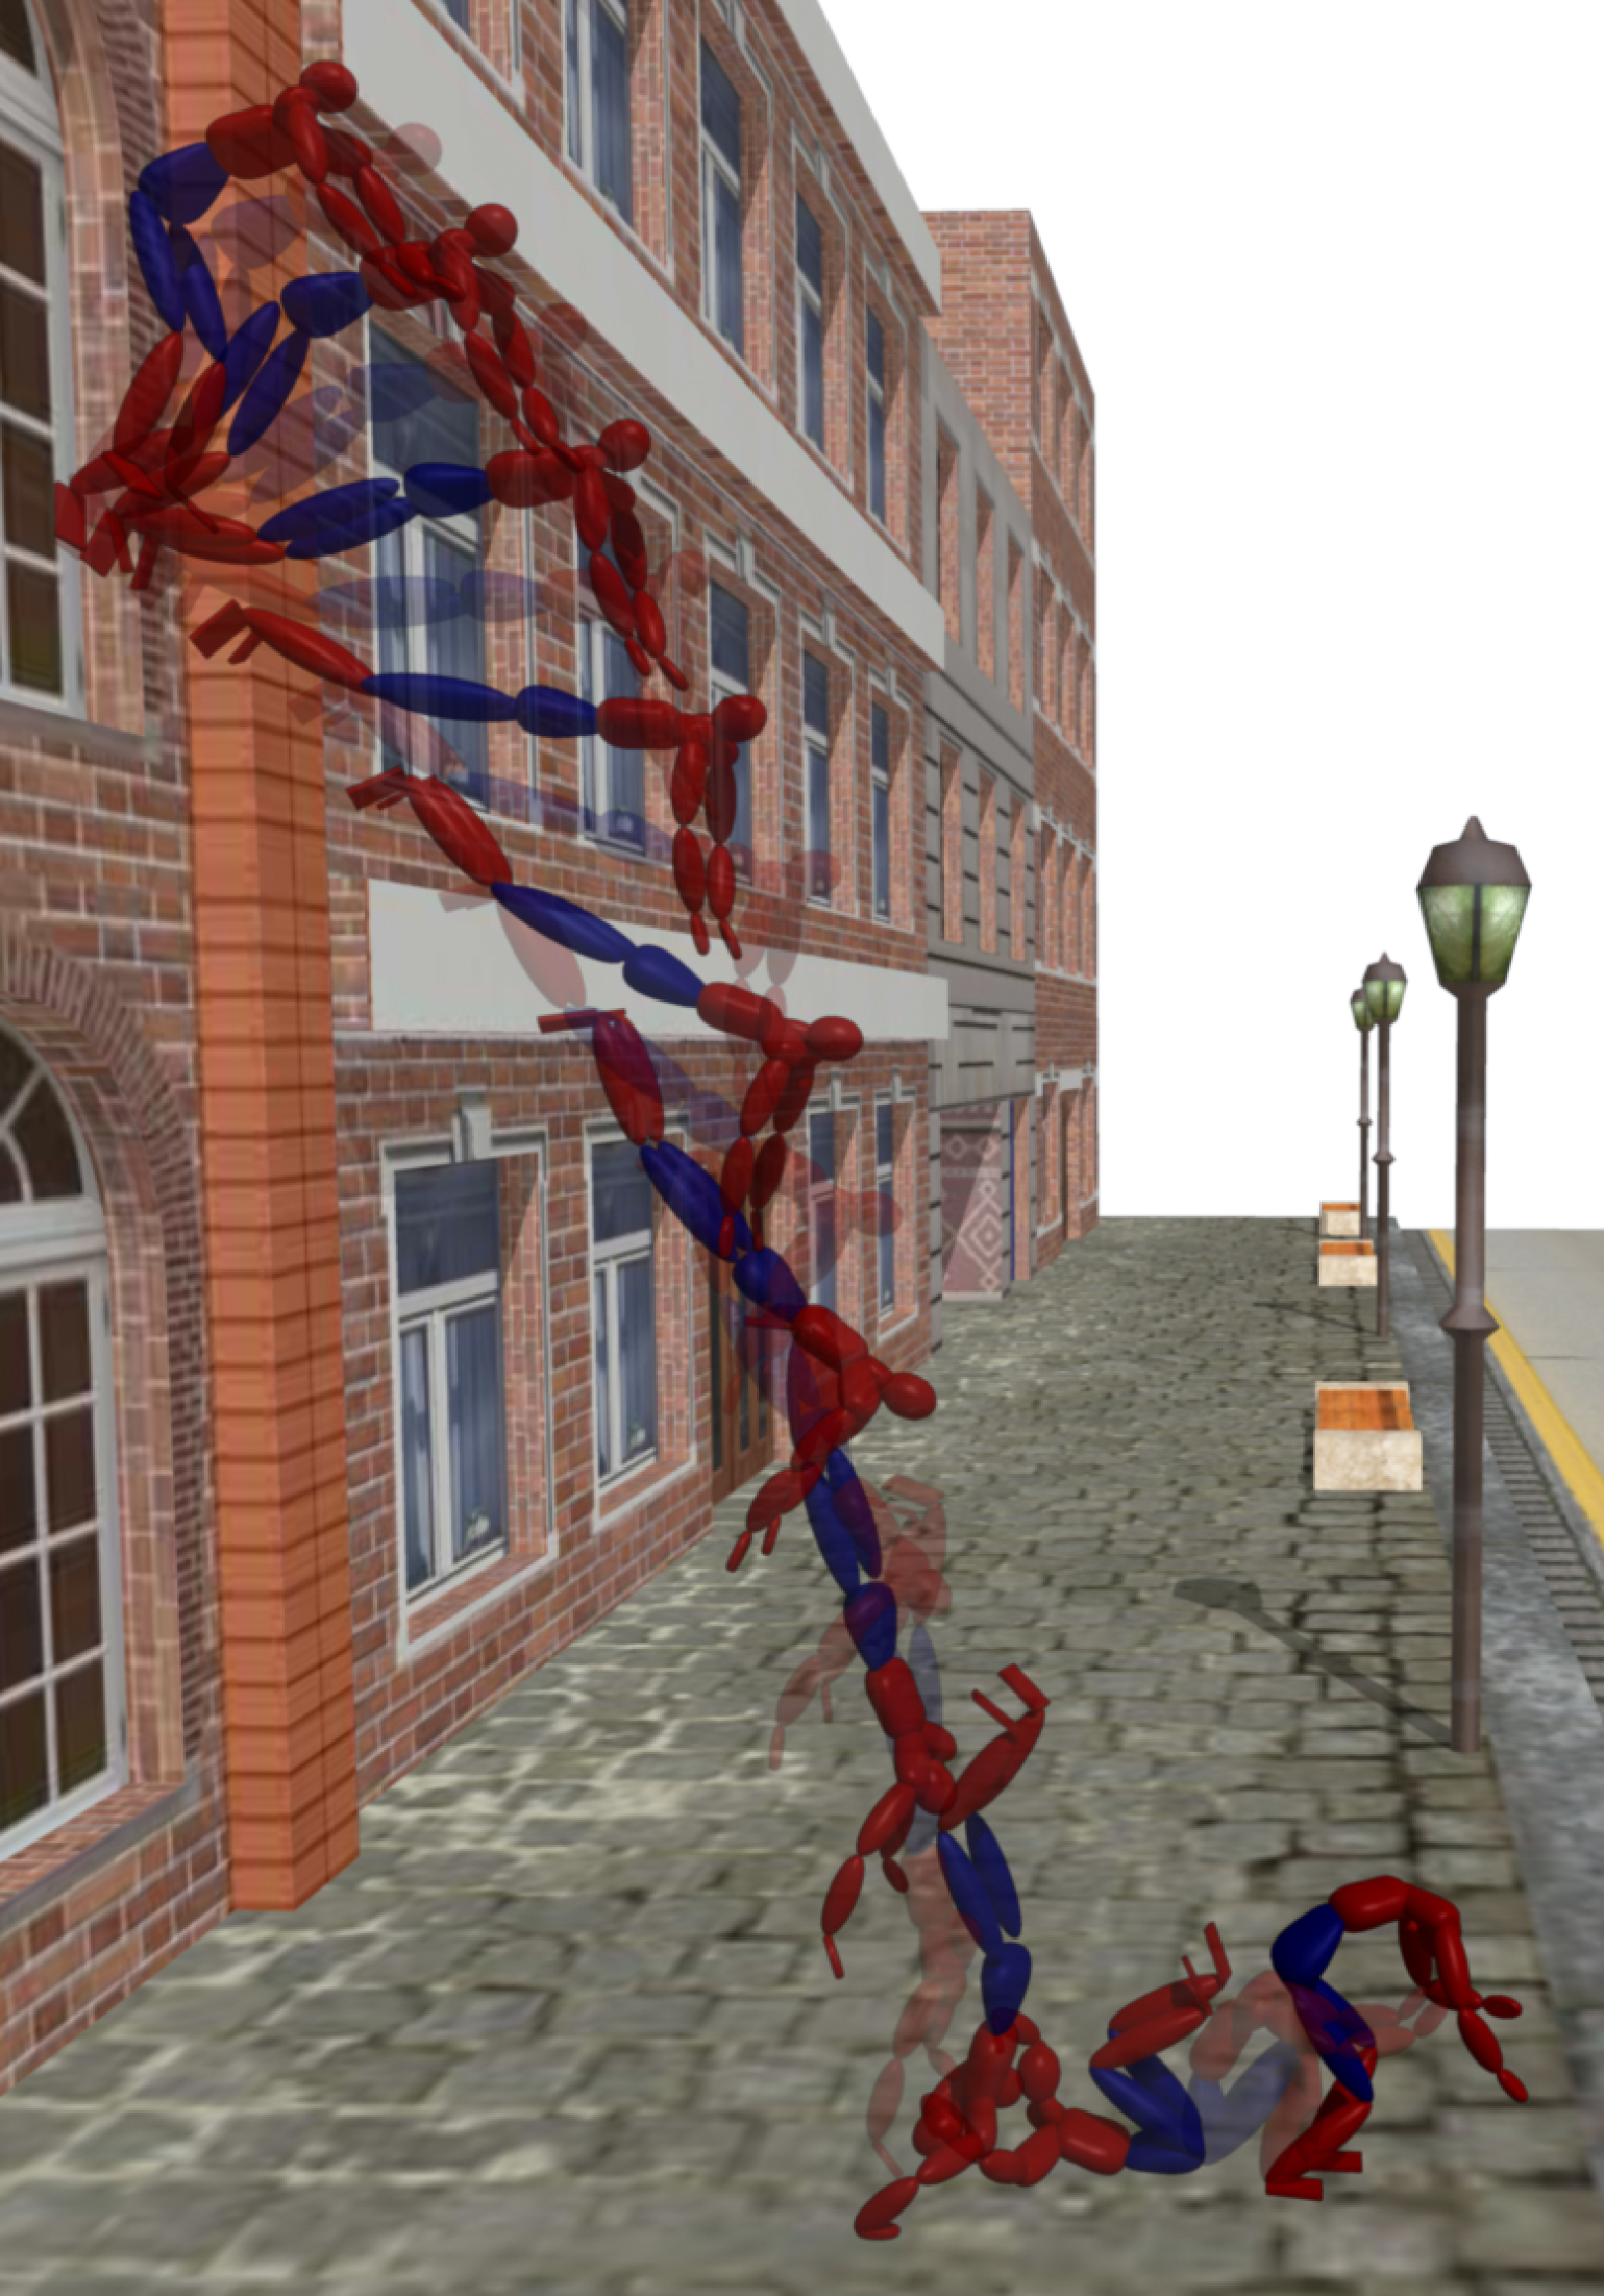
\includegraphics[width=4.0in]{images/ResultImageCol}
  \caption{Hands-first landing motion.}
  \label{fig:landing_resultHands}
\end{figure}

%% \begin{table}
%% \center
%% {
%% %% \small
%% \caption{
%%   Range of initial conditions. Top: Hands-first landing
%%   strategy. Bottom: Feet-first landing strategy.
%%   \sehoon{Statistics for success rate}
%% }
%% \begin{tabular}{|c| c|  c| c|  c| c| c|}
%% \hline
%% \label{tab:initialConditions}
%%   & {\small \textbf{y}}{\tiny(m)} 
%%   & {\small \textbf{$v_z$}}\tiny{(m/s)} 
%%   & {\small\textbf{$v_x$}}{\tiny(m/s)}  
%%   & {\small\textbf{$\omega_x$}}{\tiny(Rad/s)} 
%%   & {\small \textbf{$\omega_y$}}{\tiny(Rad/s)} 
%%   & {\small \textbf{$\omega_z$}}{\tiny(Rad/s)} \\ \hline
%% {\small \textbf{Hands: min}} & {\small 2.0 } & {\small 0.0} & {\small -1.0} & {\small 0.0} & {\small -0.5} & {\small -0.5} \\ \hline
%% {\small \textbf{Hands: max}} & {\small 10.0} & {\small 8.0} & {\small  1.0} & {\small 8.0} & {\small  0.5} & {\small  0.5} \\\hline
%% {\small \textbf{Feet: min}} & {\small 2.0 } & {\small -4.0} & {\small -4.0} & {\small -4.0} & {\small -6.0} & {\small -6.0} \\ \hline
%% {\small \textbf{Feet: max}} & {\small 10.0} & {\small  8.0} & {\small  4.0} & {\small  8.0} & {\small  6.0} & {\small  6.0} \\ \hline
%% \end{tabular}
%% }
%% \end{table}

\begin{table}
\center
{
%% \small
\caption{
  Initial conditions of the examples shown in the video (in order of appearance)
}
\begin{tabular}{| c| c|  c| c|  c| c| c|}

\hline

\multicolumn{7}{|c|}{\small Hands-first landing strategy} \\ \hline

  {\small \textbf{$\vec{C}_y$}}{\tiny(m)} 
  & {\small \textbf{$v_x$}}{\tiny(m/s)}  
  & {\small \textbf{$v_y$}}{\tiny(m/s)}  
  & {\small \textbf{$v_z$}}\tiny{(m/s)} 
  & {\small \textbf{$\omega_x$}}{\tiny(Rad/s)} 
  & {\small \textbf{$\omega_y$}}{\tiny(Rad/s)} 
  & {\small \textbf{$\omega_z$}}{\tiny(Rad/s)} \\ \hline


{\small 10.6} & {\small 0.0} & {\small 0.0} & {\small 4.0} & {\small 8.7} & {\small 0.0} & {\small 0.0} \\ \hline
{\small 5.8} & {\small 0.0} & {\small 0.0} & {\small 2.3} & {\small 5.0} & {\small 0.0} & {\small 0.0} \\ \hline
{\small 10.6} & {\small 0.0} & {\small 0.0} & {\small 6.0} & {\small 2.5} & {\small 0.0} & {\small 0.0} \\ \hline
{\small 2.5} & {\small 0.0} & {\small 0.4} & {\small 8.0} & {\small 5.0} & {\small 0.0} & {\small 0.0} \\ \hline

\hline

\multicolumn{7}{|c|}{\small Feet-first landing strategy}   \\\hline

  {\small \textbf{$\vec{C}_y$}}{\tiny(m)} 
  & {\small \textbf{$v_x$}}{\tiny(m/s)}  
  & {\small \textbf{$v_y$}}{\tiny(m/s)}  
  & {\small \textbf{$v_z$}}\tiny{(m/s)} 
  & {\small \textbf{$\omega_x$}}{\tiny(Rad/s)} 
  & {\small \textbf{$\omega_y$}}{\tiny(Rad/s)} 
  & {\small \textbf{$\omega_z$}}{\tiny(Rad/s)} \\ \hline


{\small 6.0} & {\small 0.0} & {\small 0.0} & {\small 5.0} & {\small 4.0} & {\small -1.0} & {\small -5.8} \\ \hline
{\small 2.7} & {\small 0.0} & {\small -1.0} & {\small 0.0} & {\small 0.0} & {\small 0.0} & {\small 0.0} \\ \hline
{\small 5.5} & {\small 1.0} & {\small 0.0} & {\small 0.0} & {\small 0.0} & {\small 5.0} & {\small 0.0} \\ \hline
{\small 9.6} & {\small -2.0} & {\small 0.0} & {\small -3.5} & {\small 0.9} & {\small 2.1} & {\small -3.9} \\ \hline

\end{tabular}
\label{tab:landing_initialConditions}
}
\end{table}


To evaluate the generality of our algorithm, we simulated landing
motions with a wide range of initial conditions (Table
\ref{tab:landing_initialConditions}), various landing styles (hands-first, feet-first,
consecutive rolls), and different skeleton models. We also demonstrated that
our algorithm is robust to unpredicted runtime perturbations and
different physical properties of the landing surface. Please see the
accompanying video to evaluate the quality of our results.


\paragraph{Feet-first landing strategy.} The most recommended landing
strategy from freerunning community is the feet-first landing. Our
results verify that the feet-first landing strategy is indeed very
robust for falls with arbitrary linear and angular momentum. There are
two key advantages of using feet as the first point of contact. First,
average human has longer and stronger legs than arms. Using legs to
land provides more time and strength to compress and absorb vertical
impact. Second, the feet-first strategy has an additional thrusting
step after compression and before rolling stage. During the thrusting
step, the character can utilize the contact forces to drastically
change the linear and angular velocity in preparation for rolling. Our
results show that a successful forward roll can be carried out even
when the character is falling with backward and lateral linear
velocity or nonplanar angular velocity.
%% (Figure \ref{fig:resultFeet}).

For the feet-first strategy, the coefficients of the landing condition in
Equation (\ref{eqn:landing_approxLandingAngle}) are: $a = -0.01, b = -0.06, c =
-0.03$, and $d = 0.45$. When the character transitions to the rolling
stage, we specified an asymmetric ready-to-roll pose to increase the
visual appeal of the motion.

\paragraph{Hands-first landing strategy.}
Using hands as the first point of contact can generate visually
pleasing stunts (Figure \ref{fig:landing_resultHands}). For falls with
dominant planar velocity ($v_z$ and $\omega_x$), the hands-first
strategy performs as well as the feet-first strategy. However, when
the initial condition has large lateral linear momentum or angular
momentum in yaw and roll axes, the hands-first strategy becomes less
robust. Unlike the feet-first strategy, which has an additional
thrusting step, the hands-first strategy is unable to change forward
direction drastically after landing. This imposes stringent conditions
on the contact forces because, in order to roll successfully, the
contact forces must counteract non-planner momentum, while stopping
downward momentum and maintaining forward momentum. Such forces
usually violate the unilateral constraint of ground reaction force.

For the hands-first strategy, the coefficients of the landing condition
are: $a = -0.01, b = -0.06, c = -0.03$, and $d = 3.08$. Note that the
coefficients are identical to those of the feet-first strategy except
for the constant term, indicating that the gradient of the angle of
attack with respect to the landing velocity is the same between
feet-first and hands-first landing strategies. 
%% We used a symmetric ready-to-roll pose for the hands-first strategy
%% because it reduces the chance of spinning and sideway rolling.

\paragraph{Consecutive rolls.}
Once the character starts rolling, it is rather effortless to continue
on. By looping the end of the rolling stage back to the beginning, we
showed that the character was able to make two consecutive rolls to
break a fall with large forward speed. Falling on multiple surfaces is
also easy to simulate using our controller. One example demonstrated a
continuous sequence of the character landing on the roof of a car,
leaping forward, landing again on the sidewalk, and finishing with a
dive roll (Figure \ref{fig:landing_teaser}). With our controller, a variety of
impressive action sequences can be generated easily without any
recorded or pre-scripted motions.
\begin{figure}[ht]
\center
  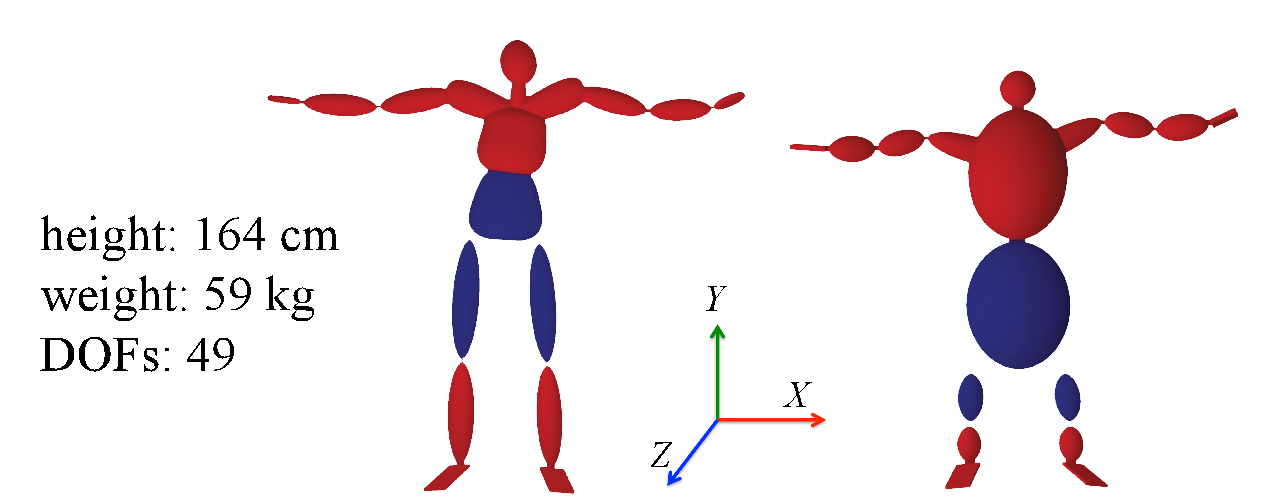
\includegraphics[width=4.2in]{images/diffSkel1}
  \caption{
    Left: The character model used for most examples. Right: A
    character with a disproportionately large torso and short legs.
  }
 \label{fig:landing_models}
\end{figure}
\paragraph{Different skeleton models.}
The character model we used to generate most examples has a height of
$164$cm, a weight of $59$ kg, and $49$ DOFs. The controllers designed
for this character can be applied to a drastically different character
whose torso is twice as long and twice as wide, comparing to the
default character. It also has very short legs and a small head
(Figure \ref{fig:landing_models}). We tested both hands-first and feet-first
landing strategies on this new character. The results are similar in
quality to the default character, although the new character hits its
head on the ground because it is difficult to tuck the head with such
a short neck.
All the control parameters remain the same for the second
character, except for $\bar{c}_y$ increasing by  $5cm$ and the
desired landing angle increasing by $0.25 rad$.


\paragraph{Runtime perturbations.}
One great advantage of physical simulation is that the outcome can be
altered on the fly based on user interactions. We demonstrated the
interactivity of our simulation in two different ways. First, the user
can directly ``drag'' the character to a different location or
orientation when the character is in the air. This example shows off
robustness and efficiency of our airborne controller. As the character
being relocated, it starts to recalculate and finds a new plan to
execute in real-time. Second, we let the user shoot cannons at the
character as a source of external forces. When a cannon hits the
character, it exerts force and torque on the character, causing a
passive response followed by active replanning and execution.

\paragraph{Different landing surfaces.}
We tested our controller on surfaces with different elasticities and
friction coefficients. When the character lands on an elastic surface,
such as a gymnastic floor or a trampoline, the character tumbles in
the air instead of rolling on the ground. We generated a continuous
sequence where the character stopped the fall on an elastic surface by
tumbling three times and finishing with a forward roll. This example
shows that various interesting acrobatic sequences can be
generated by simply concatenating our falling and rolling controllers
repeatedly. In another example, we reduced the friction coefficient to
simulate an icy surface. The character was able to use the same control
algorithm to roll, but failed to stand up at the end.

\subsection{Evaluation}

\paragraph{Performance.}
All the results shown in the video were produced on a single core of
3.20GHz CPU. Our program runs at $550$ frames per second. The
bottleneck of the computation is the optimization routine in the
airborne controller. We use Open Dynamic Engine to simulate the
character. The time step is set at $0.2$ millisecond, and runs
the airborne optimization in 50 Hz.
\begin{figure}[ht]
\center
  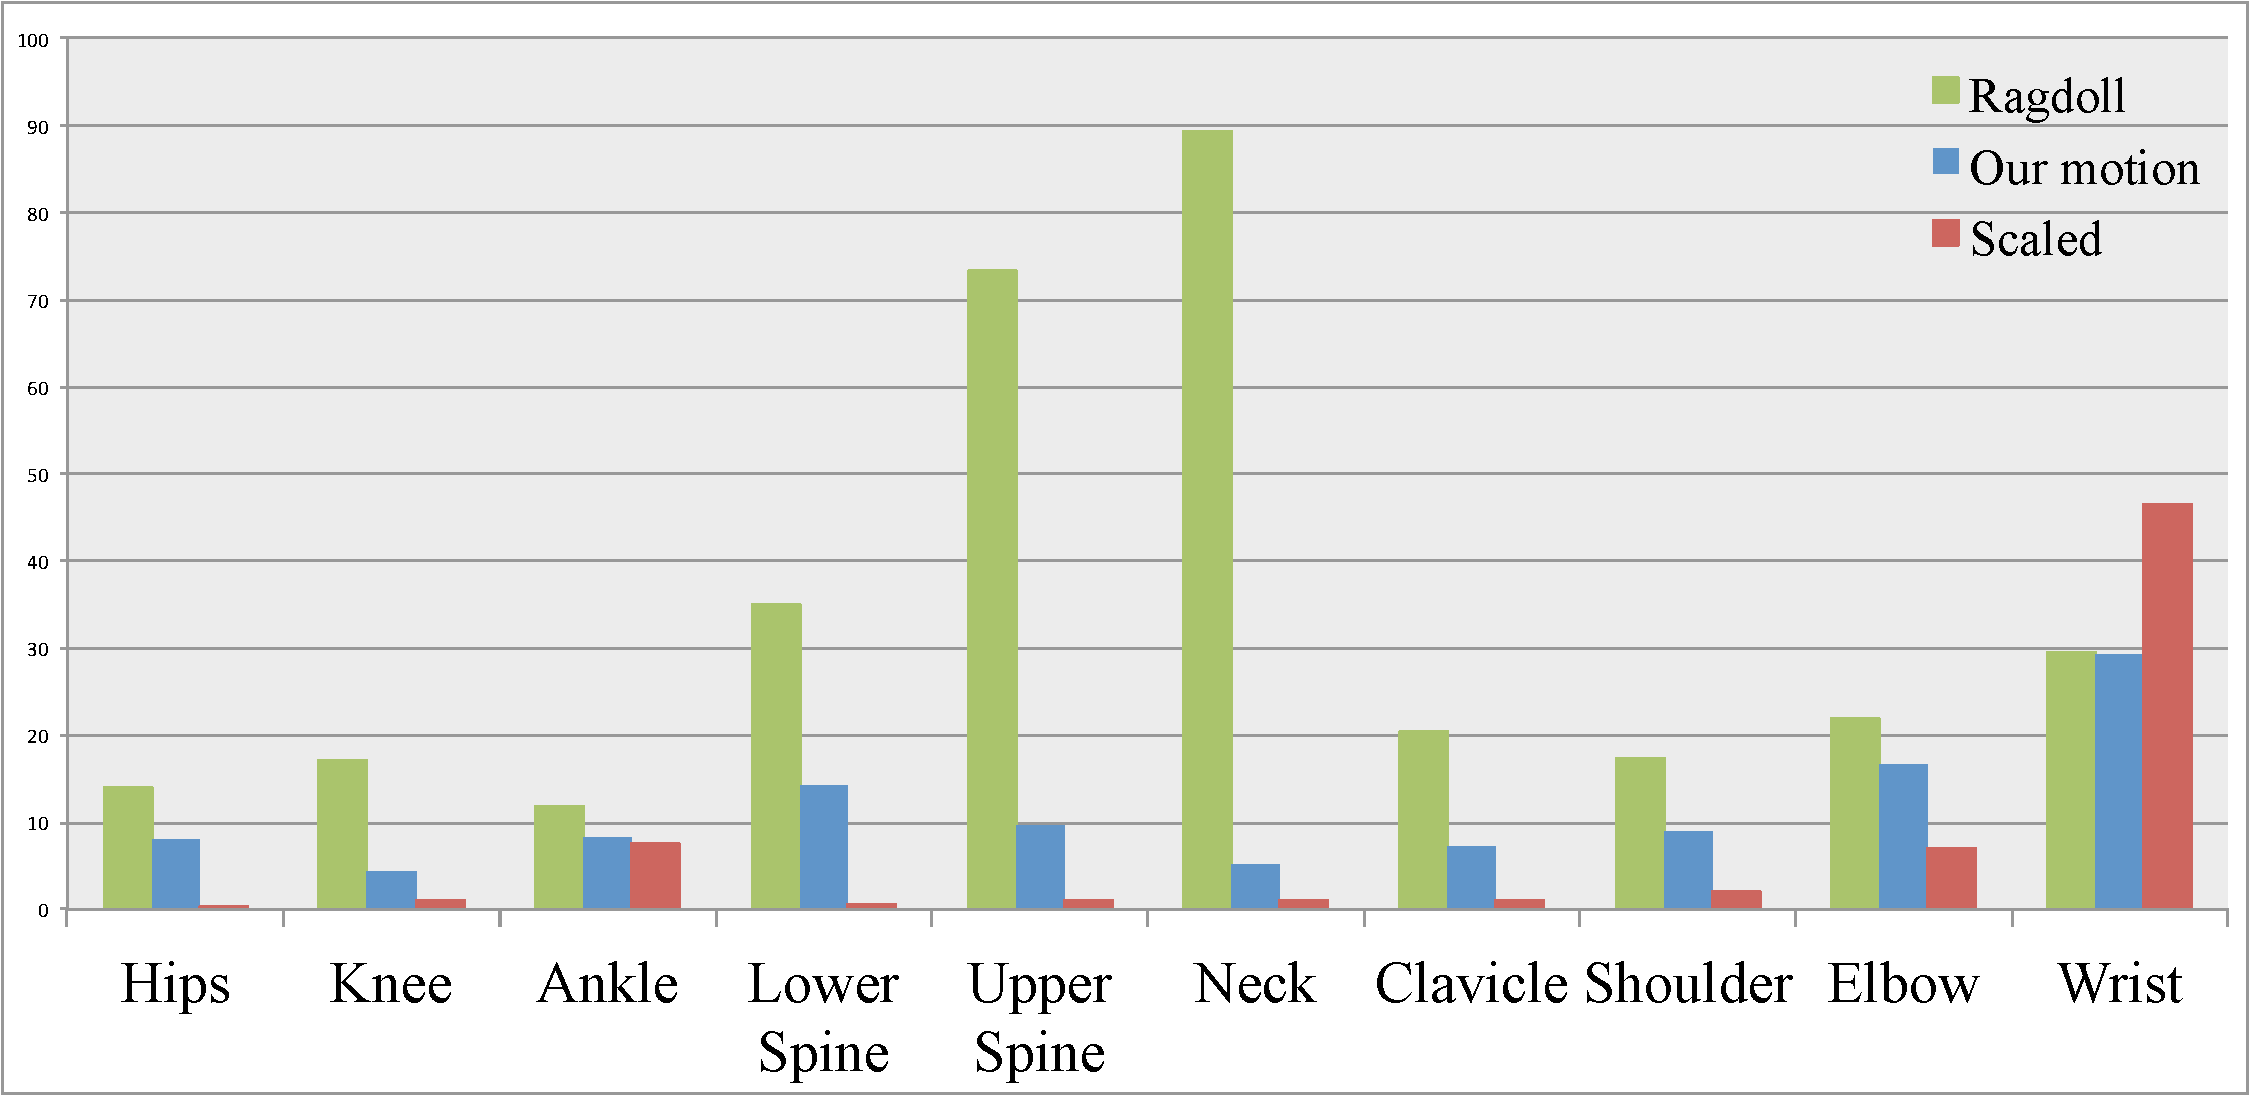
\includegraphics[width=4.2in]{images/stress}
  \caption{
    Maximal stress for each joint from a hands-first landing
    motion. Results are quantitatively similar across all of our
    simulations. Green: Ragdoll motion. Blue: Our motion. Orange: Joint
    stress scaled by mass.}
%% \karen{Order of three bars: Green, blue,
%%       and orange. The joint names from left to right: Hip, Knee,
%%       Ankle, Lower spine, Upper spine, Neck, Clavicle, Shoulder,
%%       Elbow, and Wrist.}
 \label{fig:landing_jointStress}
\end{figure}
\paragraph{Joint stress.}
We approximated joint stress as the constraint force that holds two
rigid bodies together at a joint. For each joint, we computed the
maximal joint stress during the landing phase (Figure
\ref{fig:landing_jointStress}). We observed that, in most trials, the joints
which endure the most impact are those connected to contacting
end-effectors (\ie hands or feet). The spine joints (lumbar and
thoracic vertebrae) and hip joints are also subject to large
impact. However, when we scaled each joint by the total mass it
supports (\eg the hip joint supports the mass of the entire leg), we
found that the joint stress has low variance across the entire
character's body, with the exception of the joints near the
end-effectors.
%% \begin{table}
%% \center
%% {
%% %% \small
%% \caption{Joint Stress Comparison}

%% \begin{tabular}{c  c c}
%% \label{tab:jointStress}
%%  } & \textbf{Ragdoll} & \textbf{Our controller} \\ \hline

%% \textbf{Neck}     & 73.26 &  9.74   \\ \hline
%% \textbf{Spine}    & 35.09 & 14.14   \\ \hline
%% \textbf{Shoulder} & 20.30 &  7.35   \\ \hline
%% \textbf{Hips}     & 13.98 &  7.91   \\ \hline
%% \end{tabular}
%% }
%% \end{table}


When we compared the joint stress between our motion and a passive
ragdoll motion with the same initial condition, the ragdoll motion
caused much more damage on the neck and the spine (Figure
\ref{fig:landing_jointStress}). In fact, the only joints that endured similar
amount of stress were those used for the first point of contact (\eg
wrists or ankles). These results validate that our controller indeed
produces safer landing motion and protects important body parts. We
repeated the experiments for different initial conditions.  In the
worst case of our experiments, the average joint stress is still four
times lower than landing as a passive ragdoll. The data also show that
our controller generates less damaging landing motion even when the
character cannot roll successfully, such as dropping from $20$ meters.


\paragraph{Comparison with video footages.}
We compared our simulated motion side-by-side with a collection of
video footages (\cite{APR:2011:URL}).  The simulations are based on the
same landing strategy and our best guess of the initial conditions from
the videos. Although it is not possible to achieve identical motions,
results show that our motion is qualitatively similar to the video
footages.

\subsection{Limitations}
The main limitation of our work is the lack of balance control after
the character stands up. There are many existing balance control
algorithms we could implement. However, we chose to defer the
implementation until we decide on what the character's next action
should be. In the freerunning scenario, the character transitions to
running motion seamlessly right after a roll. If freerunning is our goal, we
would modify the current get-up control algorithm to provide more
forward thrust. Other possibilities of the next action include
walking, stepping, jumping, or standing still. Different next actions
will result in different balance strategies. Ideally, a character
should be equipped with motor skills to execute all different balance
strategies and autonomously determines which strategy to execute, but
this is considered out of the scope of this work.

Another limitation is the predefined landing pose for each landing
strategy. This inflexibility can negatively affect the character's
ability to adapt to different environments. For example, if the
character lands on a narrow wall, the landing pose needs to be
adjusted on the fly. One possible solution is to use a simple inverse
kinematics method to compute desired joint angles before landing.

